%%%%%%%%%%%%%%%%%%%%%%%%%%%%%%%%%%%%%%%%%%%%%%%%%%%%%%%%%%%%%%%%%%%%%%%%%
% This file is part of the LaTeX sources of the OMDoc 1.6 specification
% Copyright (c) 2008 Michael Kohlhase
% This work is licensed by the Creative Commons Share-Alike license
% see http://creativecommons.org/licenses/by-sa/2.5/ for details
% The source original is at https://github.com/KWARC/OMDoc/doc/spec 
%%%%%%%%%%%%%%%%%%%%%%%%%%%%%%%%%%%%%%%%%%%%%%%%%%%%%%%%%%%%%%%%%%%%%%%%%

\begin{omgroup}[creators=miko,id=spec-intro]{The \omdoc Format}

In this chapter we will discuss issues that pertain to the general setup of the \omdoc
format, before we present the respective modules in later chapters. {\omdocv{1.6}} is the
first step towards a second version of the \omdoc format.


\begin{omgroup}[id=syntax-semantics]{Dimensions of Representation in \omdoc}
\begin{newpart}{re-read and strengthen the argumentation}
\begin{wrapfigure}r{8.5cm}\vspace*{-1em}
\fbox{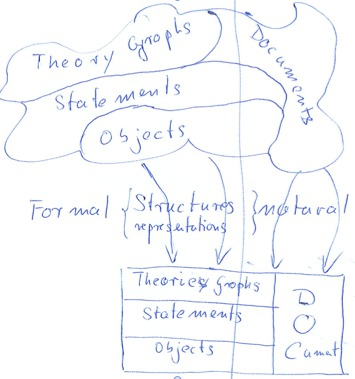
\includegraphics[width=8.2cm]{../figures/omdoc-dimensions}}
\caption{Dimensions of Representation in \omdoc}\label{fig:dimensions}\vspace*{-1em}
\end{wrapfigure}
\paragraph{Strict vs. Pragmatic} The \omdoc format is divided into two sub-languages:
``Strict'' \omdoc (in the lower half of Figure~\ref{fig:dimensions}) and ``Pragmatic''
\omdoc (in the upper half\ednote{add the words ``strict'' and ``pragmatic'' to the
  picture}). The first subset uses a minimal set of elements representing the meaning of a
mathematical expression in a uniform structure, while the second one tries to strike a
pragmatic balance between verbosity and formality. Both forms of content expressions are
legitimate and have their role in representing mathematics. The strict \omdoc format
features a minimal set of conceptually orthogonal representational primitives, resulting
in expressions with canonical structure, which simplifies the implementation of \omdoc
processors as well as the comparison of content expressions.  The pragmatic \omdoc
format provides a large representational infrastructure that aims at being intuitive for
humans to understand, read, and write.\ednote{maybe state the numbers of elements in the
  end} In particular, the simplicity and conceptual clarity of strict \omdoc allow to
express structural well-formedness constraints, whereas the vocabulary of pragmatic \omdoc
is much nearer to mathematical practice and is thus easier to learn. It is a crucial
design choice of the \omdoc format that the meaning fo pragmatic representations is
defined entirely interms of strict representations\footnote{The strategy of dividing a
  markup format into a simple and structurally elegant core language and a larger set of
  pragmatic extensions which can be given a meaning by translating into the core was first
  pioneered by the author for content {\mathml}3~\cite{CarlisleEd:MathML08}}. Note that
there may be multiple ``pragmatic vocabularies'' defined in terms of the strict core
catering to different communities and their tastes.

The introduction of strict \omdoc and the re-interpretation of pragmatic \omdoc in
terms of it is radical redesign of the \omdoc format, which is new in {\omdocv{1.6}}.
For this reason we consider {\omdocv{1.6}} the first step into the direction of
{\omdocv{2}}. With the development of strict \omdoc we aim to identify the
representational primitives for representing mathematical documents, which can be given a
simple and elegant semantics.

\paragraph{Formal vs. Informal} 

One of the hallmarks of mathematical language is that is very rigorous in structure and
usage in an attempt to fix the meaning of (mathematical) objects and statements about
them. Indeed, the first decades of the last century established that mathematical language
can in principle be expanded into logical form, where all objects and statements are fully
identified by their syntactic form, and all reasoning steps are similarly justified by
their form alone. we speak of ``formal mathematics'', when this is exercised and of
``formal reasoning'', when proofs are carried out in logical systems on this basis . In
the last decades, significant parts of mathematical knowledge have been formalized and
verified with the help of computers. But formalization and formal reasoning is still so
costly and tedious that only a very small part of mathematics is formalized and verified
in practice. Currently almost all mathematical documents consist of a mix of formal and
informal (i.e. natural language) elements --- certainly during the development of
mathematical knowledge, but also in publications. Therefore are representation format for
mathematical documents must allow this as well, consequently, \omdoc has two
sub-languages, ``formal \omdoc'' (on the left side of Figure~\ref{fig:dimensions}) and
``natural \omdoc'' (on the right side).

\omdoc offers markup at three levels: objects, statements, and context.
\begin{compactdesc}
\item[objects] are usually represented as {\emph{formulae}} or \emph{natural language
    phrases} in mathematical documents. In formal \omdoc formulae are marked up according
  to their functional structure (as operator trees) and according to their layout in
  informal \omdoc (as layout trees). Note that any object can be represented in all three
  ways and all three ways of representation can be mixed at any level to account for
  mathematical practice, e.g. for mixed formulae like $\{n\in\mathbb{N}\bigl|n>3 \;\text{
    is prime}\}$.
\item[statements] are usually represented as \emph{natural language sentences (with
    formulae)}\footnote{or even larger text fragments made up of sentences like
    paragraphs} in informal settings and as (logical) formulae in formal ones. The
  discussion about the three ways of representation of objects applies analogously. Note
  that functional markup in formal \omdoc only addresses part of the requirements of
  formality, since their meaning depends on their context; we will explore this next.
\item[theory graphs] The context of objects (and the statements that contain
  them) is given by special statements (declarations). For conciseness and tractability,
  \omdoc groups declarations into ``theories'' and connects them by ``theory morphisms''
  into ``theory graphs''. In a nutshell, every object (and thus every statement) has a
  ``home theory'', in which is meaningful. Theory morphisms make objects and statements
  available in their target theories. 
\end{compactdesc}
As statements, theories and theory graphs are large objects, their informal
representations (as mathematical text fragments and documents) usually carry linguistic
cues to their discourse structure\ednote{change the ``documents'' in
  Figure~\ref{fig:dimensions} to ``discourse'', at least in the strict box}. We discuss
the relation between the discourse structure of informal representations and the formal
structure of statements and theory graphs next.

\paragraph{Discourse vs. Content Structure}

Mathematical Documents are very explicitly structured to help the reader grasp the complex
objects, their relationships, and the flow of the argumentation in the proofs: Objects are
often represented as formulae that reveal their structure, statements are labeled by
indicators to their epistemic contribution to context (e.g. by labeling them as
``definitions'' or ``theorems'') and numbered for exact reference. The exposition of
larger documents usually follows a topical structure with superimposed narrative structure
driven by knowledge dependencies rather than e.g. a temporal dramaturgy driven by
suspense.  Even so, the structure of an informal document may be quite different from the
formal structure of the knowledge it introduces. For instance, when we introduce a new
concept in a course, we often first introduce a naive reduced approximation $\mathcal{N}$
of the real theory $\mathcal{F}$, only to show an example $\mathcal{E_N}$ of where this is
insufficient. Then we propose a first (straw-man) solution $\mathcal{S}$, and show an
example $\mathcal{E_S}$ of why this does not work. Based on the information we gleaned
from this failed attempt, we build the eventual version $\mathcal{F}$ of the concept or
theory and demonstrate that this works on $\mathcal{E_F}$.

\begin{wrapfigure}l{7cm}
  \infigures{content_vs_narrative}
\caption{Content vs. Narrative Structures}\label{fig:straw-man}
\end{wrapfigure}
The structure with the solid lines and boxes at the bottom of {\myfigref{straw-man}}
represents the content structure, where the circles $\mathcal{N}$, $\mathcal{E_N}$,
$\mathcal{S}$, $\mathcal{E_S}$, $\mathcal{F}$, and $\mathcal{E_F}$ signify theories for
the content of the respective concepts and examples. The arrows represent the
{\twintoo{theory}{inheritance}} structure, e.g. Theory $\mathcal{F}$ imports theory
$\mathcal{N}$. The top part of the diagram with the dashed lines stands for the narrative
structure, where the arrows mark up the document structure. For instance, the slides
$\text{sl}_i$ are grouped into a lecture. In the example in {\myfigref{straw-man}}, the
second slide of ``lecture'' presents the first example: the text fragment $\text{n}_1$
introduces it, and $\text{n}_2$ presents $\mathcal{E_N}$ and $\text{n}_2$ might say
something like ``this did not work in the current situation, so we have to extend the
conceptualization\ldots''. In a conventional setting, the narrative structure on the top
and the content structure would be represented in different documents: The lecture slides
and the formalization, and the equivalences (e.g. that $\text{n}_2$ verbalizes
$\mathcal{E_N}$; we have visualized these relations as dotted arrows in
{\myfigref{straw-man}}) could not be taken advantage of, since they are not explicitly
represented.

\begin{wrapfigure}r{7cm}\vspace*{-1em}
\infigures{adp}
\caption{The Active Documents Paradigm}\label{fig:adp}\vspace*{-1em}
\end{wrapfigure}
But these equivalences can be utilized to render services to the reader, for instance the
imports relation in the theory graph on the lower half of Figure~\ref{fig:straw-man}
induces a dependency relation that can be used to generate a minimal explanation (without
the motivation) of $\cE_\cF$.  For an example at the object level, consider for instance
the formula $a(x+y^2)$, whose layout is ambiguous in two places: $a$ could be a factor in
a product (presented as juxtaposition) or a function that is applied to an
argument. Likewise $y^2$ could be the variable $y$ raised to the second power or the
second element in the sequence $y^1,y^2,\ldots,y^n$. Humans can usually disambiguate this
from the context, but a screen reader service needs access to the operator tree to read
this as ``$a$ times [pause] $x$ plus $y$ squared'' or ``$a$ applied to [pause] $x$ plus
$y$ two''.

\omdoc aims to reconcile the dichotomy between discourse structures (in informal
mathematical documents which currently carry most of mathematical knowledge) and formal
structures (that machines can operate upon) in one joint format. The central technique
employed in \omdoc is that of ``parallel markup'': The technique comes from MathML, where
the \element{semantics} element is used to accomodate equivalent layout (presentation
{\mathml}) and operator trees (content {\mathml}) and possibly foreign
representations. Equivalence of nested sub-structures are represented by special
cross-references.  The \mathml processor choses the one most adequate to its task --- in
the absence of distinguisthing information the first child.

\omdoc extends this to the document level: The document contains elements whose children
are alternative representations of the same object/statement/theory.\ednote{implement
  this, and think about the cross-referencing, also need continuations to break tree
  overlaps, e.g. in content objects straddling slides.} The significance of this is

for that is Figure~\ref{fig:adp} shows the \ednote{talk about parallel markup, content
  documents and narrative documents and how to crosslink them and share structure}.


Just as for content-based systems on the formula level, there are now MKM systems that
generate presentation markup from content markup, based on general presentation
principles, also on this level. For instance, the {\sc{ActiveMath}}
system~\cite{MelBue:krma03} generates a simple narrative structure (the
presentation; called a personalized book) from the underlying content structure (given in
\omdoc) and a user model.

\paragraph{Coverage} 
Currently our understanding of these primitives is largely limited to formal parts of
mathematics, therefore strict {\omdocv{1.6}} covers significantly less of informal
mathematical documents than {\omdocv{1.2}}, so the meaning-giving translation from
pragmatic \omdoc elements to strict \omdoc is partial. We plan to develop strict
\omdoc into a system with greater coverage in the upcoming versions of \omdoc.
{\omdocv{2.0}} will be the first stable version where the coverage of strict \omdoc is
complete.
\end{newpart}
\end{omgroup}

\begin{omgroup}[id=spec-intro.modular]{\omdoc as a Modular Format}

A modular approach to design is generally accepted as best practice in the development of
any type of complex application. It separates the application's functionality into a
number of "{\indextoo{building blocks}}" or "{\indextoo{module}s}", which are subsequently
combined according to specific rules to form the entire application. This approach offers
numerous advantages: The increased {\indextoo{conceptual clarity}} allows developers to
share ideas and code, and it encourages reuse by creating well-defined modules that
perform a particular task. Modularization also reduces complexity by decomposition of the
application's functionality and thus decreases debugging time by localizing errors due to
design changes. Finally, flexibility and maintainability of the application are increased
because single modules can be upgraded or replaced independently of others.

The \omdoc vocabulary has been split by thematic role, which we will briefly overview in
{\myfigref{omdoc-modules}} before we go into the specifics of the respective modules in
{\srefl{mobj}{quiz}}. To avoid repetition, we will introduce some attributes already in
this chapter that are shared by elements from all modules. In {\sref{document-model}} we
will discuss the \omdoc document model and possible sub-languages of \omdoc that only
make use of parts of the functionality (\sref{sub-languages}).

\begin{myfig}{omdoc-modules}{The \omdoc Modules}
\begin{small}
\begin{tabular}{|l|l|l|l|}\hline
  Module & Title & Required? & Chapter\\\hline\hline
  {\presbf\MOBJmodule{spec}} &  Mathematical Objects & yes & {\sref{mobj}}\\\hline
    \multicolumn{4}{|p{11cm}|}{\presem Formulae are a central part of mathematical
       documents; this module integrates the content-oriented representation
       formats {\openmath} and {\mathml} into \omdoc}\\\hline\hline
  {\presbf\MTXTmodule{spec}} &  Mathematical Text & yes & {\sref{mtext}}\\\hline
    \multicolumn{4}{|p{11cm}|}{\presem Mathematical vernacular,
  i.e. natural language with embedded formulae}\\\hline\hline
  {\presbf\DOCmodule{spec}} & Document Infrastructure & yes & {\sref{omdoc-infrastructure}}\\\hline
    \multicolumn{4}{|p{11cm}|}{\presem  A basic infrastructure for
      assembling pieces of  mathematical knowledge into functional documents and 
      referencing their parts }\\\hline\hline
  {\presbf\METAmodule{spec}} &  Metadata & yes &   {\srefs{dc-elements}{dc-roles}}\\\hline
    \multicolumn{4}{|p{11cm}|}{\presem Contains bibliographical and licensing metadata 
      (``{\twintoo{data}{about data}}'') 
      which can be used to annotate many \omdoc elements by descriptive and
      administrative information that facilitates navigation and organization}\\\hline\hline 
  {\presbf\RTmodule{spec}} & Rich Text Structure & no & {\sref{rt}}\\\hline
    \multicolumn{4}{|p{11cm}|}{\presem Rich text structure in
  mathematical vernacular (lists, paragraphs, tables, \ldots)}\\\hline\hline
  {\presbf\STmodule{spec}} &  Mathematical Statements & no  & {\sref{statements}}\\\hline
    \multicolumn{4}{|p{11cm}|}{\presem Markup for mathematical forms like 
      {\indextoo{theorem}s},  {\indextoo{axiom}s}, {\indextoo{definition}s}, 
      and {\indextoo{example}s} that can be used to specify or define properties
      of given mathematical objects and theories to group mathematical
  statements and provide a notion of context.}\\\hline\hline
  {\presbf\PFmodule{spec}} &  Proofs and proof objects & no & {\sref{proofs}}\\\hline 
    \multicolumn{4}{|p{11cm}|}{\presem Structure of proofs
     and argumentations at various levels of details and formality}\\\hline\hline
  {\presbf\ADTmodule{spec}} &  Abstract Data Types & no & {\sref{adt}}\\\hline 
    \multicolumn{4}{|p{11cm}|}{\presem  Definition schemata for
      sets that are built up inductively from constructor symbols}\\\hline\hline 
  {\presbf\CTHmodule{spec}} & Complex Theories & no & {\sref{complex-theories}}\\\hline
    \multicolumn{4}{|p{11cm}|}{\presem Theory morphisms; they can be used
    to structure mathematical theories}\\\hline\hline
  {\presbf\DGmodule{spec}} & Development Graphs & no & {\sref{development-graphs}}\\\hline
    \multicolumn{4}{|p{11cm}|}{\presem Infrastructure for managing theory
  inclusions, change management}\\\hline\hline
  {\presbf\EXTmodule{spec}} & Applets, Code, and Data & no & {\sref{ext}}\\\hline
    \multicolumn{4}{|p{11cm}|}{\presem Markup for applets, program code,
  and data (e.g. images, measurements, \ldots)}\\\hline\hline
  {\presbf\PRESmodule{spec}} & Presentation Information & no &  {\sref{pres}}\\\hline
    \multicolumn{4}{|p{11cm}|}{\presem Limited functionality for
    specifying presentation and notation information for local typographic
      conventions  that cannot be determined by general principles alone}\\\hline\hline
  {\presbf\QUIZmodule{spec}} &  Infrastructure for Assessments & no & {\sref{quiz}}\\\hline
    \multicolumn{4}{|p{11cm}|}{\presem Markup for exercises integrated
    into the \omdoc document model}\\\hline 
  \end{tabular}
\end{small}
\end{myfig}
The first four modules in {\myfigref{omdoc-modules}} are required (mathematical documents
without them do not really make sense), the other ones are optional. The
document-structuring elements in module {\DOCmodule{spec}} have an attribute
{\attributeshort{modules}} that allows to specify which of the modules are used in a
particular document (see {\sref{omdoc-infrastructure}} and
{\sref{sub-languages}}).
\end{omgroup}

\begin{omgroup}[id=omdoc-ns]{The OMDoc Namespaces}

The namespace for the {\omdocv2} format is the \atwinalt{URI}{OMDoc}{namespace}{URI}
\url{http://omdoc.org/ns}. Note that the \omdoc \twinalt{namespace}{OMDoc}{namespace}
does not reflect the versions\footnote{The namespace is different from the {\omdocv1}
  formats (versions 1.0, 1.1, and 1.2), which was
  {\snippet{http://www.mathweb.org/omdoc}}, but the {\omdocv2} namespace will stay
  constant over all versions of the {\omdocv2} format.}, this is done in the
{\attributeshort{version}} attribute on the {\twintoo{document}{root}} element
\element{omdoc} (see {\sref{omdoc-infrastructure}}).  As a consequence, the
\omdoc vocabulary identified by this namespace is not static, it can change with each
new \omdoc version. However, if it does, the changes will be documented in later
versions of the specification: the latest released version can be found
at~\cite{URL:omdocspec}.

In an \omdoc document, the \omdoc namespace must be specified either using a
{\twintoo{namespace}{declaration}} of the form
{\snippet{xmlns="}}\url{http://omdoc.org/ns}{\snippet{"}} on the \element{omdoc} element
or by prefixing the {\twintoo{local}{name}s} of the \omdoc elements by a namespace
prefix (\omdoc customarily use the prefixes {\snippet{omdoc:}} or {\snippet{o:}}) that
is declared by a {\atwintoo{namespace}{prefix}{declaration}} of the form
{\snippet{xmlns:o="}}\url{http://omdoc.org/ns}{\snippet{"}} on some element dominating the
\omdoc element in question (see {\extref{book}{xml}} for an introduction). \omdoc also
uses the following namespaces\footnote{In this specification we will use the
  {\twintoo{namespace}{prefix}es} above on all the elements we reference in text unless
  they are in the \omdoc namespace.}:

\begin{scriptsize}
  \begin{center}
    \begin{tabular}{|l|l|l|}\hline
      Format      & namespace URI & see \\\hline\hline
      Dublin Core & \url{http://purl.org/dc/elements/1.1/} &   {\srefs{dc-elements}{dc-roles}}\\\hline
      Creative Commons & \url{http://creativecommons.org/ns} & {\sref{creativecommons}}\\\hline
      {\mathml} & \url{http://www.w3.org/1998/Math/MathML} & {\sref{cmml}}\\\hline
      {\openmath} & \url{http://www.openmath.org/OpenMath} & {\sref{openmath}}\\\hline
      {\xslt} & \url{http://www.w3.org/1999/XSL/Transform} & {\sref{pres}}\\\hline
    \end{tabular}
  \end{center}
\end{scriptsize}
Thus a typical document root of an \omdoc document looks as follows:
  \begin{lstlisting}[mathescape]
<?xml version="1.0" encoding="utf-8"?>
<omdoc xml:id="test.omdoc" version="1.6"
  xmlns="http://omdoc.org/ns"
  xmlns:cc="http://creativecommons.org/ns"
  xmlns:dc="http://purl.org/dc/elements/1.1/"
  xmlns:om="http://www.openmath.org/OpenMath"
  xmlns:m="http://www.w3.org/1998/Math/MathML">
$\ldots$
</omdoc>
\end{lstlisting}  
\end{omgroup}

\begin{omgroup}[id=common-attribs]{Common Attributes in OMDoc}

Generally, the \omdoc format allows any attributes from foreign (i.e. non-\omdoc)
\twinalt{namespaces}{foreign}{namespace} on the \omdoc elements. This is a commonly
found feature that makes the {\xml} encoding of the \omdoc format extensible. Note
that the attributes defined in this specification are in the default (empty)
\twinalt{namespace}{default}{namespace}: they do not carry a namespace prefix. So any
attribute of the form {\snippet{na:xxx}} is allowed as long as it is in the scope of a
suitable {\atwintoo{namespace}{prefix}{declaration}}.

Many \omdoc elements have optional {\attributeshort[ns-attr=xml]{id}} attributes that
can be used as identifiers to reference them. These attributes are of type
\twinalt{\snippet{ID}}{type}{ID}, they must be unique in the document which is important,
since many {\xml} \twinalt{applications}{XML}{application} offer functionality for
referencing and retrieving elements by \twinalt{{\snippet{ID}}-type}{type}{ID} attributes.
Note that unlike other {\snippet{ID}}-attributes, in this special case it is the name
{\attributeshort[ns-attr=xml]{id}}~\cite{XML:id05} that defines the
{\indextoo{referencing}} and {\indextoo{uniqueness}} functionality, not the type
declaration in the {\indextoo{DTD}} or {\twintoo{XML}{schema}} (see
{\extref{book}{xml.validation}} for a discussion).

  Note that in the \omdoc format proper, all {\twintoo{ID}{type}} attributes are of the
  form {\attributeshort[ns-attr=xml]{id}}. However in the older {\openmath} and {\mathml}
  standards, they still have the form {\attributeshort{id}}. The latter are only
  recognized to be of type {\snippet{ID}}, if a document type or {\xml}schema is
  present. Therefore it depends on the application context, whether a DTD should be
  supplied with the \omdoc document.

  For many occasions (e.g. for printing \omdoc documents), authors want to control a
  wide variety of aspects of the presentation. \omdoc is a content-oriented format, and
  as such only supplies an infrastructure to mark up content-relevant information in
  \omdoc elements. To address this dilemma {\xml} offers an interface to 
  {\twintoo{Cascading}{Style Sheet}s} ({\css})~\cite{BosHak:css98}, which allow to specify
  presentational traits like {\twintoo{text}{color}}, {\twintoo{font}{variant}},
  {\indextoo{positioning}}, {\indextoo{padding}}, or {\indextoo{frame}s} of
  {\twintoo{layout}{box}es}, and even {\indextoo{aural}} aspects of the text.

  To make use of {\css}, most \omdoc elements (all that have
  {\attributeshort[ns-attr=xml]{id}} attributes) have {\attributeshort{style}} attributes
  that can be used to specify {\css} \twinalt{directives}{CSS}{directive} for them. In the
  \omdoc fragment in {\mylstref{css-basic}} we have used the \attribute{style}{omtext}
  attribute to specify that the text content of the \element{omtext} element should be
  formatted in a centered box whose width is 80\% of the surrounding box (probably the
  page box), and that has a 2 pixel wide solid frame of the specified RGB color. Generally
  {\css} directives are of the form {\snippet{A:V}}, where {\snippet{A}} is the name of
  the aspect, and {\snippet{V}} is the value, several {\css}
  \twinalt{directives}{CSS}{directive} can be combined in one {\attributeshort{style}}
  attribute as a {\twintoo{semicolon-separated}{list}} (see {\cite{BosHak:css98} and the
    emerging {\css} 3} standard).

\begin{lstlisting}[label=lst:css-basic,mathescape,
   caption={Basic {\css} Directives in a {\attributeshort{style}} Attribute},
   index={style,class}]
<?xml version="1.0" encoding="utf-8"?>
<?xml-stylesheet type="text/css" href="http://example.org/style.css"?>
<omdoc xml:id="stylish">
  $\ldots$
  <omtext xml:id="t1" style="width:80%;align:center;border:2px #006699 solid">
    <h:p>Here comes something 
      <h:span style="font-weight:bold;color:green" class="emphasize">stylish</h:span>!
    </h:p>
  </omtext>
  $\ldots$
</omdoc>
\end{lstlisting}

Note that many {\css} properties of parent elements are inherited by the children,
if they are not explicitly specified in the child. We could for instance have set
the {\twintoo{font}{family}} of all the children of the \element{omtext} element
by adding a directive {\snippet{font-family:sans-serif}} there and then override it by
a directive for the property {\snippet{font-family}} in one of the children.

Frequently recurring groups of {\css} directives can be given symbolic names in {\css}
\twinalt{styles heets}{CSS}{style sheet}, which can be referenced by the
{\attributeshort{class}} attribute. In {\mylstref{css-basic}} we have made use of this
with the class {\snippet{emphasize}}, which we assume to be defined in the style sheet
{\snippet{style.css}} associated with the document in the ``{\twintoo{style
    sheet}{processing instruction}}'' in the prolog\footnote{i.e. at the very beginning of
  the {\xml} document before the document type declaration} of the {\xml} document
(see~\cite{Clark:assxd99} for details).  Note that an \omdoc element can have both
{\attributeshort{class}} and {\attributeshort{style}} attributes, in this case, precedence
is determined by the rules for {\css} style sheets as specified in~\cite{BosHak:css98}. In
our example in {\mylstref{css-basic}} the directives in the {\attributeshort{style}}
attribute take precedence over the {\css} directives in the style sheet referenced by the
{\attributeshort{class}} attribute on the \element{phrase} element. As a consequence,
the word ``stylish'' would appear in green, bold italics.
\end{omgroup}
\end{omgroup}

%%% Local Variables: 
%%% mode: latex
%%% TeX-master: "main"
%%% End: 


% LocalWords:  omdoc mobj attribs DTD XMLSchema dtd css omtext RGB omgroup miko
% LocalWords:  lst emph xml utf stylesheet href DOCTYPE px serif ns dc attr
% LocalWords:  xmlns creativecommons cmml openmath cc om mtxt rt adt ext pres
% LocalWords:  na xxx es sans mathescape prolog omdocv wrapfigure vspace fbox
% LocalWords:  includegraphics ednote mathml compactdesc mathbb bigl indextoo
% LocalWords:  indextoo myfigref srefl sref myfig hline presbf MOBJmodule mtext
% LocalWords:  presem MTXTmodule DOCmodule METAmodule srefs twintoo RTmodule
% LocalWords:  ldots STmodule PFmodule ADTmodule CTHmodule DGmodule EXTmodule
% LocalWords:  PRESmodule QUIZmodule attributeshort atwinalt twinalt omdocspec
% LocalWords:  atwintoo extref scriptsize xslt lstlisting mylstref assxd99
